%!TeX spellcheck = en_GB
%!TEX TS-program = xelatex
%!BIB TS-program = biber

\chapter{Thermal Analysis of Continuous Fibres}\label{chap:p1}

\section*{Statement of Contribution}
	This chapter includes a co-authored journal paper. The bibliographic details of the published paper are:
\begin{itemize}
	\item Javanbakht, Z, Hall, W \& Öchsner, A (2016), “Automatized Estimation of the Effective Thermal Conductivity of Carbon fibre Reinforced Composite Materials”, Defect and Diffusion Forum 370, pp. 177–183.
\end{itemize}
	My contribution as the corresponding author to the paper involved: undertaking literature review, classifying the necessary theoretical backgrounds and models, developing the programming code, analysing and discussing the finite element results, drawing figures, preparing tables, writing and editing the manuscript according to my supervisors’ comments.

\Zia\\
\Wayne\\
\vfill
\newpage
% --------------------------------------------------------------------------------------------------
\paragraph{Title} Automatised Estimation of the Effective Thermal Conductivity of Carbon fibre Reinforced Composite Materials

\paragraph{Abstract} In the current study, the representative volume element (RVE) is used to model randomly generated nanocomposite structures consisting of carbon nanotubes (CNTs) embedded in an epoxy resin matrix. The finite element Method is utilized for numerical simulations and investigation of the influential parameters on the generated RVEs. In order to automatise the whole procedure---from generating the finite element models to conducting the analyses---a subroutine-based programming approach is adopted using the MSC~Marc finite element package and Fortran programming language. The simulations can successfully predict the increase in thermal conductivity of CNT-reinforced nanocomposites by increasing the fibre volume fraction.

\paragraph{Keywords} Finite element method; Reinforced composites; Thermal conductivity; Carbon nanotubes.



\section{Introduction}
	Exceptional physical and mechanical properties of carbon nanotubes have directed a huge amount of research since their first encounter in 1991~\autocite{Iijima.1991}. Properties such as high Young's and shear moduli, low density, high thermal conductivity, and ballistic electronic conduction have introduced a wide variety of applications for CNTs in mechanics, electronics, and energy systems among other fields~\autocite{Jorio.2008}. For instance,  some single-walled nanotubes can have elastic modulus and strengths to mass ratios of approximately 19 and 56 times those of typical structural steel, respectively~\autocite{Baughman.2002}. In terms of their thermal conductivity, values above~$2000\,\sfrac{\text{W}}{\text{m}\cdot\text{K}}$ are quite common while extremely high values such as $6600\,\sfrac{\text{W}}{\text{m}\cdot\text{K}}$ have also been reported~\autocite{Berber.2000,Han.2011b}. 

	The limited thermal conductivity of polymers, specially in the amorphous ones, contrasts with their industrial applications, e.g., as heat sinks~\autocite{Han.2011b}. This makes polymers preferable mediums for fillers such as CNTs to make up nanocomposites with superior properties. In addition, direct characterization of CNTs is quite limited and thus, to avoid the obstacles of direct measurement of their thermal conductivity, experiments are conducted on the aligned nanotubes which are dispersed in a matrix~\autocite{Ruoff.1995,Thostenson.2001}.

	Due to the limitations of the experiments, numerical methods are more and more used for characterising the material properties of nanocomposites. Among these methods, the finite element method is used to simulate various physical and multi-physics phenomena among which are the transfer phenomena. Many recent researches have numerically investigated the effects of fibre aspect ratio~\autocite{Lusti.2004,Shan.2002,Afrooz.2015}, fibre orientation~\autocite{Khani.2016,Makvandi.2014b}, fibre dispersion/agglomeration~\autocite{Bakshi.2010,Hedia.2016}, interface bonding quality~\autocite{Giannopoulos.2010,Hedia.2016,Kundalwal.2012}, waviness/straightness of the fibres~\autocite{Bhuiyan.2013,Weidt.2015}, fibre volume/weight fraction~\autocite{Kundalwal.2012b,AlasvandZarasvand.2016,Chen.2004}, and property contrast among others. One of the common methods of finite element modelling is using an auxiliary scripting program, such as Python, to generate the mesh~(see~\autocite{Jafari.2011} for instance) whereas in the current study, the effects of random distributions is investigated by an automated procedure.
\section{Methodology}
	The finite element method~\autocite{Ochsner.2013,Oechsner.2016} is used in this study to simulate the heat conduction within a composite. The MSC~Marc (version 2014.2) commercial package is selected to carry out the simulations. The package provides a variety of advanced features by means of its Fortran-based subroutines, which makes it favourable for customized applications. In addition, the modules provided in~\autocite{Javanbakht.2017} are used to facilitate the programming and model generation procedures.

	The other advantage of using FORTRAN subroutines in the current study was the fact that no other programming languages, e.g., Matlab, was required for generation of the fibres. All the process was carried out using subroutines and thus, at every job submission, a newly generated fibre distribution was incorporated in the mesh. Each model generation procedure followed the steps that are denoted in Fig.~\ref{figure:flowchart}.

	\begin{figure}[!h]
	\centering
	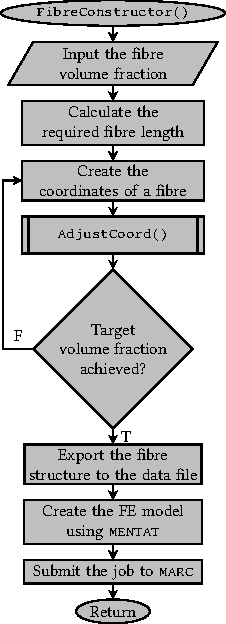
\includegraphics[scale=1]{ddf1_flow.pdf}
	\caption{Flowchart of random coordinate generation for fibres}\label{figure:flowchart}
	\end{figure}
	
	\red In the proposed flowchart, the main \code{FibreConstructor()} subroutine carries out the generation of the randomly dispersed fibres, which later will be embedded in the matrix. This subroutine aims to achieve a certain fibre volume fraction. Thus, the fibre volume fraction and the number of fibres are the given input values. Moreover, all the fibres are assumed to have the same length. For a specific fibre volume fraction and a set total number of fibres, i.e., the fixed number of 50 fibres in the current study, the length of each fibre is readily calculated. Each fibre is considered as a cylinder that is geometrically identical to a CNT; see the following paragraph for the geometrical parameters of the fibres. 
	
	After executing the two first steps of the flowchart, a loop starts to generate the pseudo-random start and end node coordinates of the fibre. In each cycle, two random coordinates are generated using the \code{GetRandNum()} function provided in~\autocite{Javanbakht.2017}. One point within the RVE (points on the faces are not allowed) and an end point are created. Then, the \code{AdjustCoord()} subroutine takes over to make sure the fibre---with the required length---is completely inside the RVE. This subroutine calculates the direction vector and the end node is relocated on this vector to satisfy the required length. If the adjusted end node is positioned within the RVE, the coordinates are confirmed. Otherwise, a new set of coordinates is created and the process flows back to adjusting the length of the fibre. The algorithm returns and the created volume fraction is tested. The loop continues until the target volume fraction is achieved. Finally, the generated fibres are inserted into the matrix without any node matching procedures, see~\autocite{marc.a} for more information. It is worth mentioning that fibre overlap is not avoided in the procedure since the discrete fibres are 2D entities for which the cross-section is not explicitly modelled.\bl

	Figure~\ref{figure:mesh1} illustrates an instance of dispersed fibres in the representative volume element. The dimensions of the RVE are $20\times20\times20\,\text{nm}^3$ and the equivalent cross sectional area of the CNTs are $1.13\,\text{nm}^2$ which was calculated based on a wall thickness of $0.34\,\text{nm}$, and an outer diameter of $1.4\,\text{nm}$~\autocite{Makvandi.2014}. The fibre volume fractions of 2.5, 5.0, 7.5, and 10\% were considered. The material properties of the matrix and fibres are shown in Table~\ref{table:ddf1_mat1}.

	\begin{figure}[t]
	\centering
	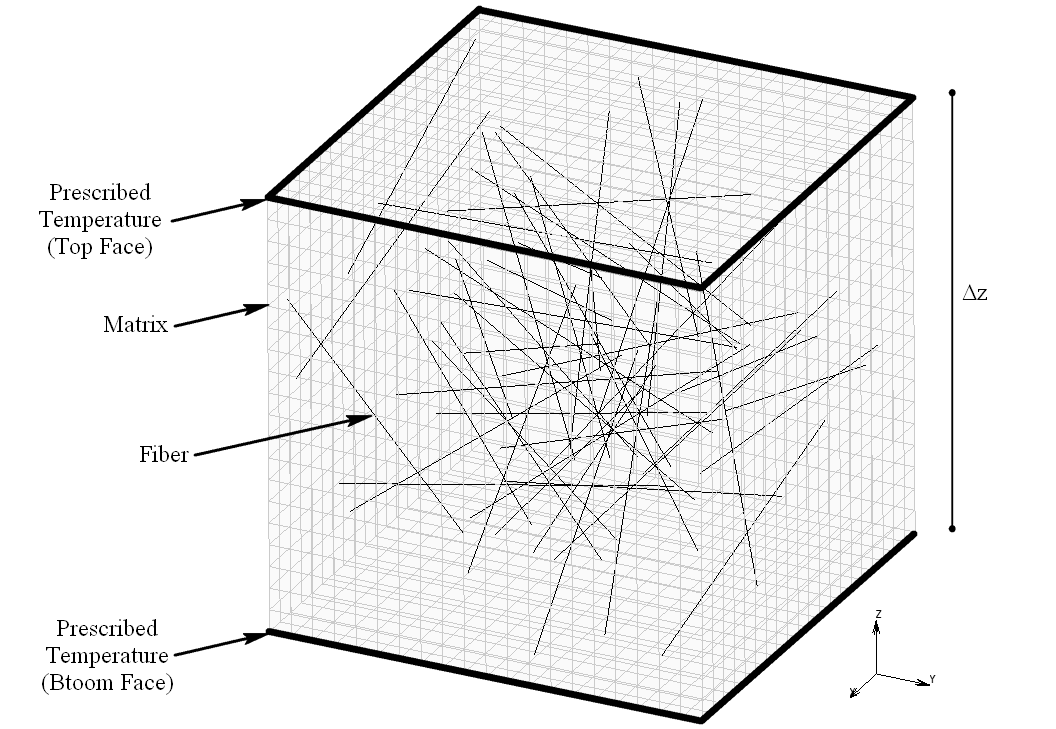
\includegraphics[width=0.8\textwidth]{random_fibres2}
	\caption{Meshed RVE with randomly distributed fibres (fibres are illustrated schematically)}\label{figure:mesh1}
	\end{figure}%

\begin{table}[!h]
\centering
\caption{Material properties of the composite components}\label{table:ddf1_mat1}
\begin{tabular}{ccc}
\toprule
\bfs{Component}&
\bfs{Material}&
\bfs{Average conductivity} ($\sfrac{\text{W}}{\text{m}\cdot\text{K}}$)\\
\toprule
Matrix&
Epoxy resin&
0.214~\autocite{Makvandi.2014}\\
Fibre&
Carbon nanotube&
2980~\autocite{Fiedler.2008}\\
\bottomrule
\end{tabular}
\end{table}%
Two types of heat transfer elements were engaged in the thermal analyses: the 8-node isoparametric hexahedral elements (type 43) consisted the mesh of the matrix and the straight 2-node link elements (type 36) were used for the fibres. A set of temperature boundary conditions were prescribed for each of the bottom and top face nodes, i.e., constant temperatures zero and 100$^\circ\text{C}$, respectively. These boundary conditions imposed a temperature gradient in the sample and generated reaction heat fluxes in the aforementioned faces. Finally, the effective thermal conductivity of the composite was calculated using Fourier's law~\autocite{Fiedler.2009}:
\begin{equation}
k=\frac{\dot{Q}}{A_0}\cdot\frac{\Delta Z}{\Delta T},\label{eq:ddf1_cond}
\end{equation}
where $k$ is the effective thermal conductivity, $\dot{Q}$ is the total reaction flux, $A_0$ is the cross-sectional area perpendicular to the flux, $\Delta Z$ is the distance between the top and bottom faces, and $\Delta T$ is the applied temperature difference.

\red
\section{Results and Discussion}
	\paragraph{Sensitivity analysis} Since the whole simulation process was automated, a sensitivity analysis was readily done. To quantify the mesh refinement in a model with only hexahedral cubic elements, the mesh density~$\gamma$ can be defined as
	\begin{equation}
		\gamma\equidef\frac{1}{\ell_\text{mesh}},
	\end{equation}
	where ($\ell_\text{mesh}$) is the characteristic dimension of the element. In the current study, several mesh densities ranging from 0.2 to 4 have been investigated where a similar rate of convergence was observed for the thermal conductivity, see Fig.~\ref{figure:sens1}. Note that the heat flux would demonstrate a similar response because of its linear relationship with the thermal conductivity, see Eq.~\eqref{eq:ddf1_cond}. The mesh density of 3, which corresponds to $0.33\times 0.33\times 0.33\,\text{nm}^3$ cubic elements, was selected for the simulations. The criterion for the selection of $\gamma=3$ was achieving a relative error percentage of below $0.05\%$.
	
\begin{figure}[!h]
\centering
%\subfloat[Total heat flux versus mesh  density]{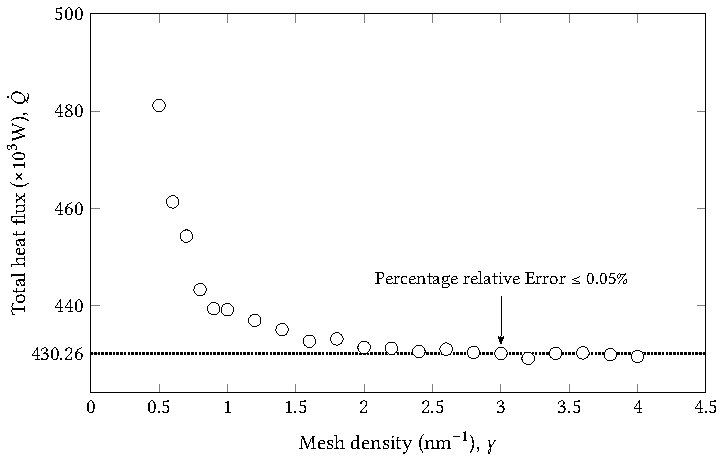
\includegraphics[scale=0.9]{ddf1_mesh_sens1}}\\
%\subfloat[Thermal conductivity versus mesh density]{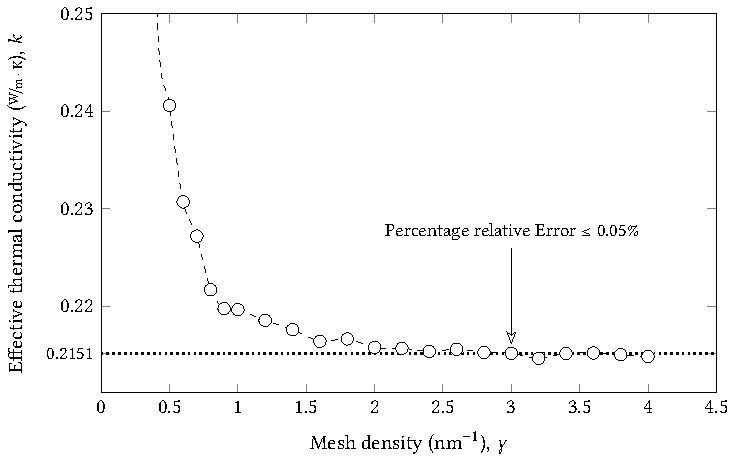
\includegraphics[scale=0.9]{ddf1_mesh_sens2}}\\
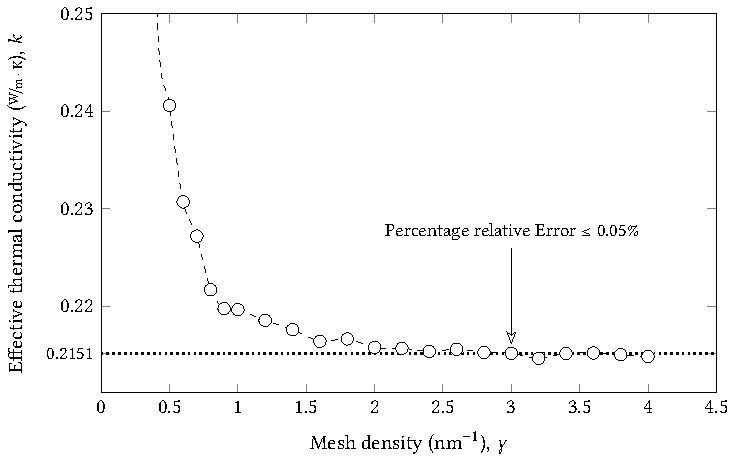
\includegraphics[scale=1]{ddf1_mesh_sens2}
\caption{\red Results of mesh sensitivity analysis for the effective thermal conductivity\bl }\label{figure:sens1}
\end{figure}%	

	\paragraph{Validation of the model}	Analytical models such as the rule of mixtures (RoM) and the inverse rule of mixtures (IRoM) provide good first estimates for upper and lower bounds of thermal conductivities of continuous fibres, respectively. In the case of random fibre orientation, the RoM is corrected with a fibre efficiency parameter for orientation ($\varkappa_\text{o}$)~\autocite{Krenchel.1964}:
	\begin{equation}
		k = \varkappa_\text{o} \zeta_\text{f}k_\text{f}+\zeta_\text{m}k_\text{m},\label{eq:ddf1_rom}
	\end{equation}
	where $\zeta$ denotes the volume fractions, $k$ is for thermal conductivities, and the `f' and `m' subscripts are used for the properties pertaining to the fibres and matrix, respectively. The efficiency of $\varkappa_\text{o}=0.2$ is a typical suggested value for randomly-oriented fibres~\autocite{Krenchel.1964}. However, nano-fibres have more pronounced properties compared to their micro counterparts, i.e., the former has very high fibre apsect ratios and there is a severe contrast between the material properties of the fibre and matrix. Although these characteristics cannot be neglected in the case of nano-fibres, they are not considered in the classic bounds such as RoM or its inverse. Therefore, the Lewis-Nielsen (LN) model~\parencite{Nielsen.1970,Nielsen.1974} was used herein:
	\begin{equation}
	    \frac{k}{k_\text{m}}=\frac{1+AB\zeta_\text{f}}{1-B\psi \zeta_\text{f}},
	\end{equation}
	with
	\begin{subequations}
	\begin{alignat}{2}
	  		A&=k_\text{E}-1,\\
	   	B&=\frac{\sfrac{k_\text{f}}{k_\text{m}}-1 }{\sfrac{k_\text{f}}{k_\text{m}}+A},\\
	   	\psi&= 1+\frac{1-\zeta_\text{f,max}}{\zeta_\text{f,max}^2}\zeta_\text{f}, 	   		
	\end{alignat}
	\end{subequations}
	where the parameter $A$ is related to the generalised Einstein's coefficient ($k_\text{E}$, intrinsic viscosity), and thus for long aligned fibres it goes towards infinity; $B$ considers the relative moduli of the inclusions and matrix and becomes unit for very high contrast properties; $\psi$ depends on the maximum packing factor of the inclusions~$\zeta_\text{f,max}$. In the literature, the value of 0.52 is proposed for maximum packing factor of inclusions, see~\autocite{Halpin.1992,Nielsen.1994}. Moreover, for the case of CNTs, where high aspect ratios are expected, the $A=8.38$ gives good results~\autocite{Kostagiannakopoulou.2016,Zimmer.2012}. 
	
	\paragraph{Results and Discussion} In Fig.~\ref{figure:ddf1_validation}, the LN model and the RoM (with 20\% efficiency) are depicted along with the obtained values from the simulations. The values of the LN model were used as benchmark values since they correspond well with the experimental values previously reported in the literature, see~\autocite{Kostagiannakopoulou.2016,Zimmer.2012}. The FE simulations were repeated to create 10 realisations per volume fraction. The mean values of the thermal conductivities were used to represent the ensemble average. All the curves commenced from the same point that corresponded to the pure matrix ($\zeta_\text{f}=0$) and deviated further as the volume fraction increases. Although the RoM varied linearly, the LN curve and the FE results seemed to change in a nonlinear fashion.
\begin{figure}[!h]
\centering
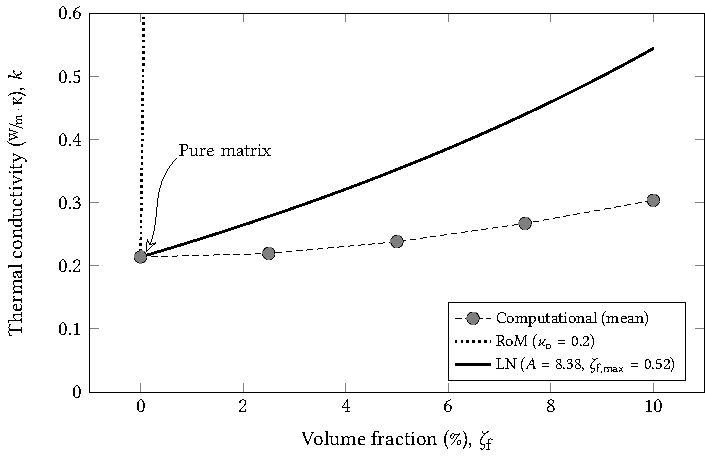
\includegraphics[scale=1]{ddf1_validation}
\caption{\red Thermal conductivity results obtained from the simulations and the Lewis-Nielson micro-model; note that the extremely large values of the RoM makes its graph out-of-proportion}\label{figure:ddf1_validation}
\end{figure}%	
	
	The ensemble mean values of the simulations are presented in Table~\ref{table:res1}. It is observed that adding CNT fibres to the matrix has altered the thermal conductivity of the composite compared to that of the pure matrix material. Namely, by increasing the fibre volume fraction, the effective conductivity of the composite increased. This trend was the same for the FE results, the LN model, and the RoM. However, the RoM highly overestimated the benchmark values whereas the FE results underestimated the thermal conductivity. The error value of the FE results also increased at higher volume fractions, which can be attributed to the elevated randomness of the model.

\begin{table}[!h]
\centering
\caption{\red Simulation results of thermal conductivity for various fibre volume fractions (10 runs per volume fraction) against the RoM and Lewis-Nielson micromechanical models; the values within the brackets are percentage relative errors}\label{table:res1}
\begin{tabular}{P{0.1\textwidth}P{0.18\textwidth}P{0.16\textwidth}P{0.22\textwidth}P{0.13\textwidth}}
\toprule
  \bfs{$\zeta_{\text{f}}$} (\%)
& \bfs{RoM + 20\% efficiency} ($\sfrac{\text{W}}{\text{m}\cdot\text{K}}$) % ($\sfrac{\text{W}}{\text{m}\cdot\text{K}}$)
& \bfs{Lewis-Nielson} ($\sfrac{\text{W}}{\text{m}\cdot\text{K}}$)
& \bfs{Average conductivity} ($\sfrac{\text{W}}{\text{m}\cdot\text{K}}$)
& \bfs{Percentage SD} % ($\sfrac{\text{W}}{\text{m}\cdot\text{K}}$)
\\\toprule
  2.5
%& $119.00 \times 10^{-6}$%0.000119
&15.11
&$2657 \times 10^{-4}$  
& $2195 \times 10^{-4}$ [17.38\%]% 0.219539
&0.1720
\\
  5.0
&30.00
&$3211 \times 10^{-4}$ 
& $2383 \times 10^{-4}$ [25.78\%]%0.238291 
%& $907.00\times 10^{-6}$%0.000907
&1.203
\\
%& $144.60\times 10^{-5}$%0.001446
  7.5
&44.90
&$3807 \times 10^{-4}$ 
& $2671\times 10^{-4}$ [29.84\%]  %0.267112
&1.712
\\
  10
%& $367.60\times 10^{-6}$%0.003676
&59.79
&$4457 \times 10^{-4}$ 
& $3038\times 10^{-4}$ [31.83\%]  %0.303779
&3.826
\\\bottomrule
\end{tabular}
\end{table}%

	Although the procedure was random, the average value of results were pretty consistent as the percentage standard deviation\,\footnote{Standard deviation normalised with respect to the mean value---it is also called percent deviation from mean value.} (SDs) were below 4\%. The percentage standard deviations increased by increasing the fibre volume fractions. Nevertheless, a very good consistency is observed. Similar to the discussed error values, the increase in inconsistency is due to the increased numerical randomness of the coordinate and orientation generation.
	
	The low values of the thermal conductivity can be attributed to the incorporated FE algorithm. The proposed automated procedure was capable of generating a range of fibre volume fractions with random orientation and spatial locations. However, as it is obvious from Fig.~\ref{figure:mesh1}, there is large matrix volume that surrounds the fibrous volume. Namely, the fibres are located more in the centre of the RVE (to avoid any collision with the boundaries). This tendency of the fibre generation procedure creates a large area with a very low conductivity, which results in low apparent thermal conductivity values. Moreover, since a fixed number of fibres, with specific geometrical properties, is accepted by the algorithm, it cannot generate very high volume fractions. This limitation should be addressed in the following releases.

\bl
	
%\begin{figure}[!h]
%\centering
%%\subfloat[Total heat flux versus various fibre volume fractions]{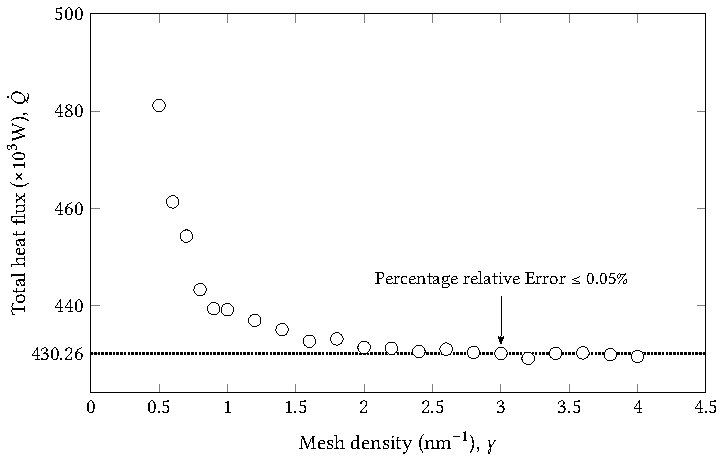
\includegraphics[scale=1]{ddf1_mesh_sens1}}\\
%%\subfloat[Thermal conductivity versus various fibre volume fractions]{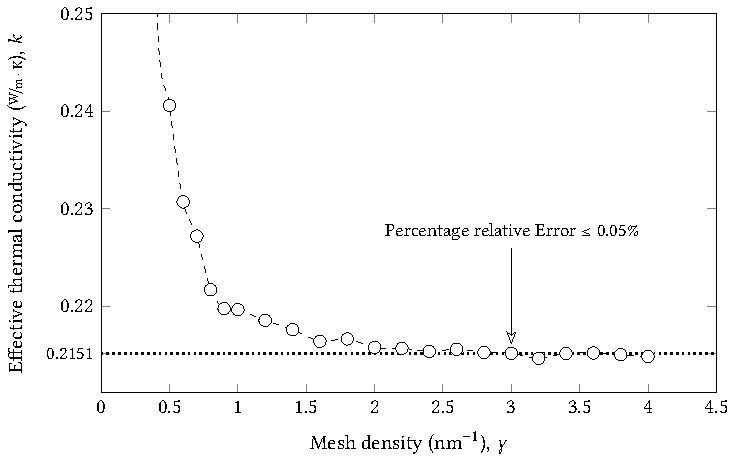
\includegraphics[scale=1]{ddf1_mesh_sens2}}\\
%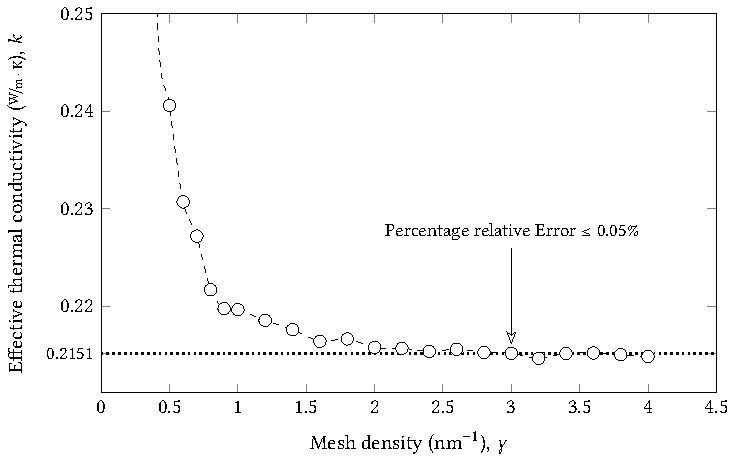
\includegraphics[scale=1]{ddf1_mesh_sens2}\\
%\caption{Thermal conductivity results obtained from the simulations (average values are based on 10 randomly generated fibre distributions at a constant fibre volume content), and Halpin-Tsai micro-model}\label{figure:result1}
%\end{figure}%

\section{Conclusion}
	In the current study, the effective thermal conductivity of randomly dispersed fibres was investigated. Random fibres (fibre volume fraction 2.5--10\%) were dispersed in every job submission by means of an automated plrocedure, which is independent of any third-party software packages. The proposed procedure generates ten pseudo-random realisations for every fibre volume fraction. Moreover, it provides more flexibility when several consecutive realisations are required, e.g., in a mesh sensitivity analysis.\red\ It was shown that by increasing the volume fractions, the effective/apparent conductivity of the RVE increases along with the corresponding error values---however, the consistency of results remained very good. Although the automated algorithm has shown a clear superiority compared to the RoM model, it still underestimates the thermal conductivity. This shortcoming is due to the tendency of the procedure to create centralised clusters of fibres surrounded by some resin-rich volumes. In future studies, this effect should be eliminated by improving the quality of the RVE, e.g., by adopting a periodic geometry, and/or releasing the fixed fibre-number constraint.\bl
	
	
%	  without regard to the aspect ratio of fibres---this corresponds to the original Halpin-Tsai formulation, see~\autocite{Halpin.1992}. Using the micro-packing principles~\autocite{Milewski.1978}, one could relate the maximum packing factor to the aspect ratio of fibres:
%	\begin{equation}
%		R=
%	\end{equation}

